\documentclass[a4paper, 12pt]{article}
\usepackage[T2A]{fontenc}
\usepackage[utf8]{inputenc}
\usepackage[english,russian]{babel}
\usepackage{amsmath, amsfonts, amssymb, amsthm, mathtools, misccorr, indentfirst, multirow}
\usepackage{wrapfig}
\usepackage{graphicx}
\usepackage{subfig}
\usepackage{adjustbox}

\usepackage{geometry}
\geometry{top=20mm}
\geometry{bottom=20mm}
\geometry{left=20mm}
\geometry{right=20mm}



\begin{document}
	\begin{titlepage}
	\begin{center}
		\large{МИНИСТЕРСТВО ОБРАЗОВАНИЯ И НАУКИ\\РОССИЙСКОЙ ФЕДЕРАЦИИ}
		
		Федеральное агентство по образованию
		\vspace{0.5cm}
		
		\large{МОСКВОСКИЙ ФИЗИКО-ТЕХНИЧЕСКИЙ ИНСТИТУТ\\(ГОСУДАРСТВЕННЫЙ УНИВЕРСИТЕТ)}
		\vspace{0.5cm}
		
		Кафедра вакуумной электроники
		\vfill
		
		{\LARGE Масс-спектроскопия остаточных газов. Квадрупольный масс-анализатор}
		\bigskip
		
		Лабораторная работа\\
		по курсу: Вакуумная электроника 
	\end{center}
	\vfill
	
	\hfill\begin{minipage}{0.4\textwidth}
		Работу выполнил\\
		студент 654 группы\\
		Нехаев Александр
	\end{minipage}
	\vfill
	
	\begin{center}
		Долгопрудный\\2018 г.
	\end{center}
	\end{titlepage}
	\tableofcontents
	\newpage
	\section{Цели и задачи исследования}
	\begin{enumerate}
		\item Ознакомиться с работой квадрупольного масс-анализатора;
		\item Исследовать масс-спектр остаточных газов в вакуумной установке;
		\item Напустить в вакуумный объем газ из баллона, исследовать масс-спектр газовой смеси;
		\item Расшифровать спектры, определить каким газам соответствует максимальное количество пиков
	\end{enumerate}
	\section{Лабораторная установка}
	\begin{figure}[h]
		\centering
		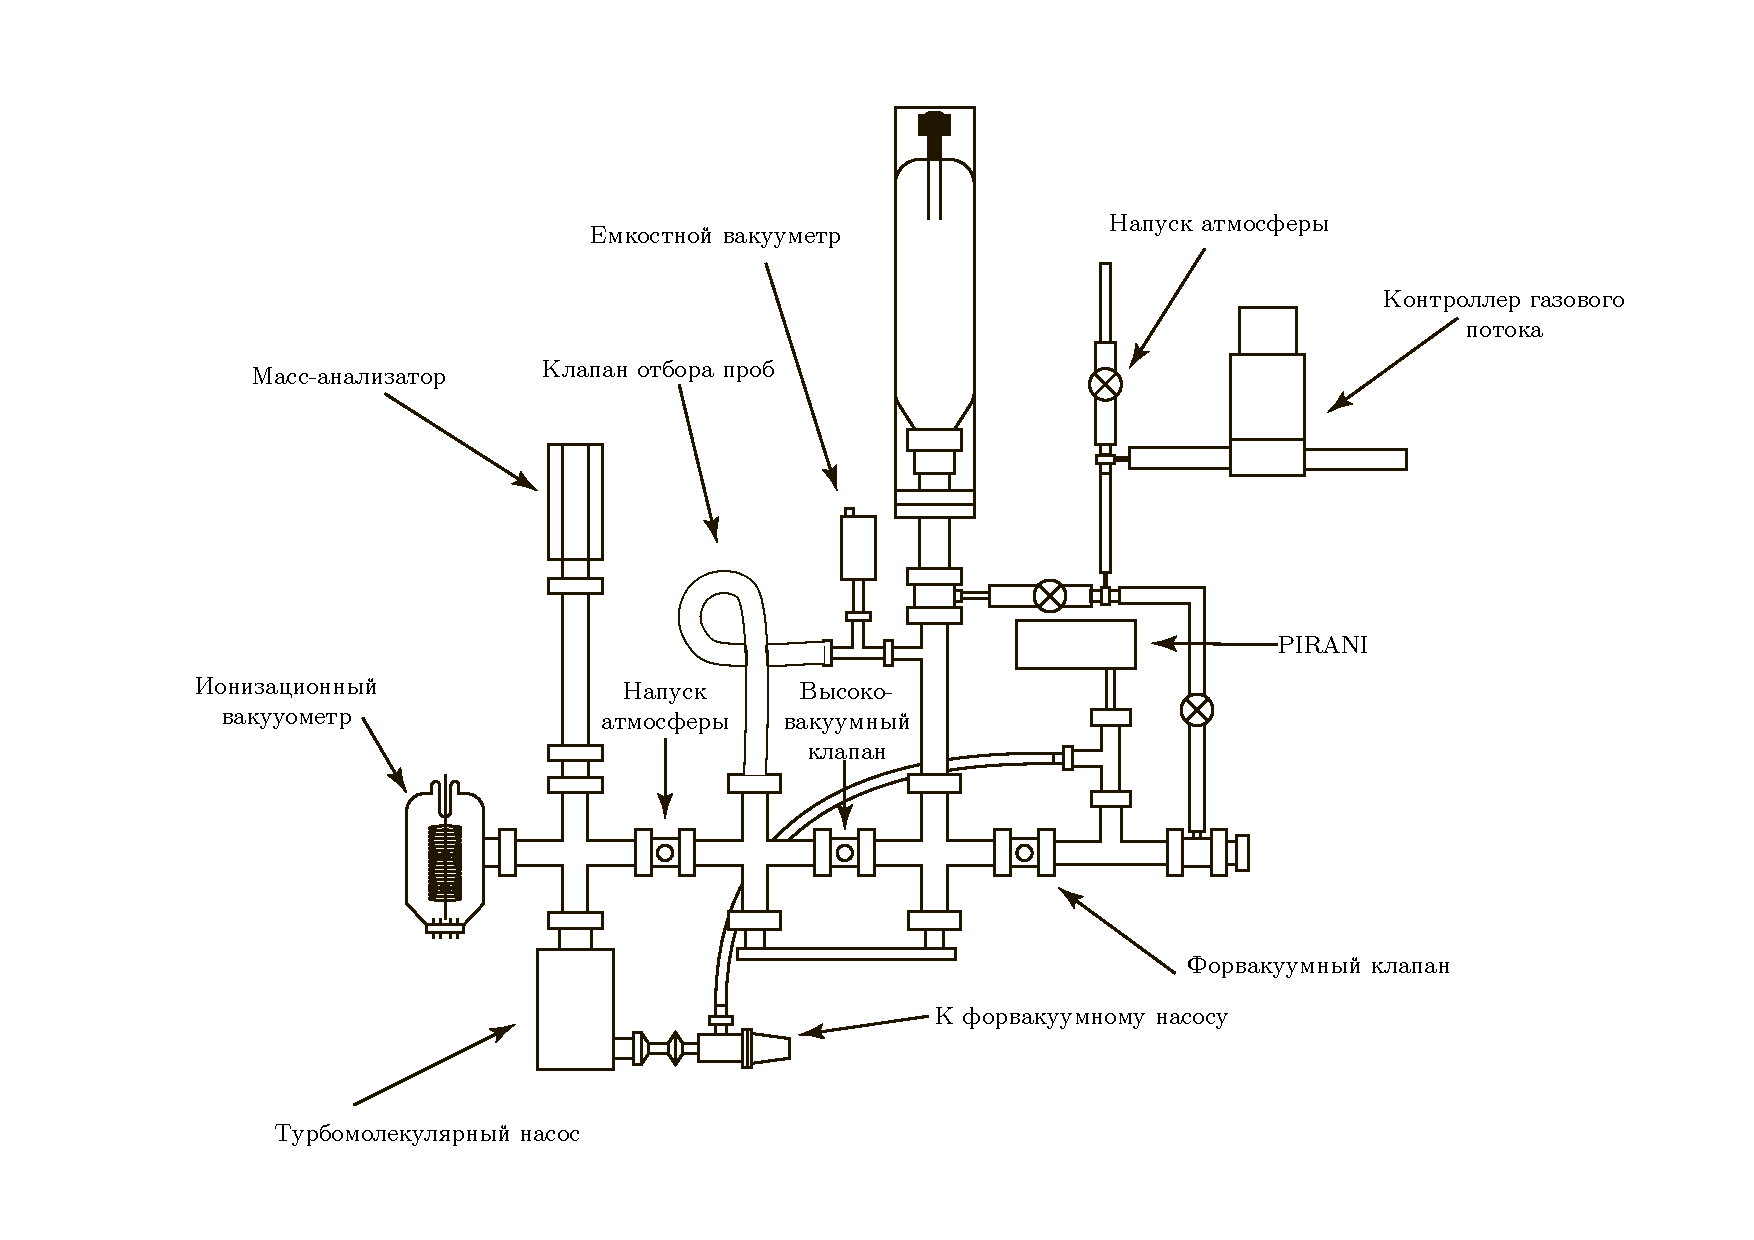
\includegraphics[scale=0.6]{MyGraph6.pdf}
		\caption{Схема лабораторной установки.}
	\end{figure}
	\newpage
	\section{Теоретическая часть}
	Масс-спектроскопия определяет массу или отношения массы иона к его заряду $(m/Z)$, а также относительное количество ионов, полученное при ионизации исследуемого вещества или уже присутствующих в изучаемой смеси. Совокупность значений $m/Z$ и относительных величин токов этих ионов, представленная в виде графика или таблицы, называется масс-спектром вещества.\par
	Приборы, в которых регистрация осуществляется электрическими методами, называются масс-спектрометрами, а приборы с регистрацией ионов на фотопластинках - масс-спектрографами. Масс-спектральные приборы состоят из источника ионов, разделительного устройства (масс-анализатора), детектора (приемника ионов), системы откачки, обеспечивающей глубокий вакуум во всей системе, и блока обработки данных (рис. \ref{idea}).\par
	\begin{figure}[h]
		\centering
		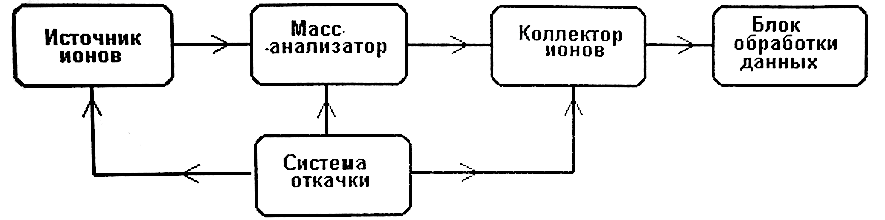
\includegraphics{idea.png}
		\caption{Блок схема масс-спектрометра}
		\label{idea}
	\end{figure}
	Масс-спектрометр работает в условиях достаточно высокого вакуума (10-5 - 10-6 Торр и выше). Создать вакуум необходимо для уменьшения рассеяния ионного пучка на молекулах остаточных газов, иначе ухудшается разрешающая способность масс-спектрометра.
	\subsection{Основные характеристики масс-спектрометров}
	\begin{enumerate}
		\item \textit{Чувствительность.} Относительную чувствительность масс-спектрометра определяется, как отношение числа зарегистрированных ионов к числу атомов введенной пробы. За абсолютный порог чувствительности принимают минимальное количество исследуемого вещества (выраженное в молях), которое доступно для регистрации в масс-спектрометре. За относительный порог принимают минимум массовой или объемной доли вещества (выраженной в \%), которые обеспечивают регистрацию выходного сигнала при отношении сигнал-шум 1:1.
		\item \textit{Разрешающая способность (R).} Она характеризует способность анализатора разделять ионы с незначительно отличающимися друг от друга массами и определяется отношением значения массы иона М к ширине его спектрального пика $\Delta М$ (выраженной в а.е.м.) на определенном уровне высоты пика (обычно 50\%): $R=M/\Delta M$. Например, R=10000 означает, что масс-анализатор может разделять ионы с массами 100,00 и 100,01 а.е.м.
	\end{enumerate}
	\subsection{Виды масс-спектрометров}
	Масс-анализаторы - это устройства для пространственно-временного разделения ионов с различными значениями $m/Z$ в магнитном или электрическом полях или их комбинациях. Различают статистические и динамические анализаторы.\par
	В статистических анализаторах ионы разделяются в постоянных или медленно меняющихся электрических и/или магнитных полях. Ионы с различными значениями $m/Z$ движутся в таком анализаторе по различным траекториям и фокусируются либо в разных точках фотопластинки, либо на узкой апертуре детектора. При плавном изменении напряженности электрического и магнитного полей анализатора происходит сканирование спектра, т.е. последовательная фокусировка на щели пучков ионов с различными значениями $m/Z$.\par
	В динамических анализаторах разделение ионов происходит под воздействием переменного электромагнитного поля с периодом изменения близким времени пролета ионов через масс-анализатор. Ионы с различными значениями m/Z разделяются, в конечном счете, по времени пролета ими определенного расстояния.
	\subsection{Квадрупольный масс-анализатор}
	\begin{figure}[h]
		\centering
		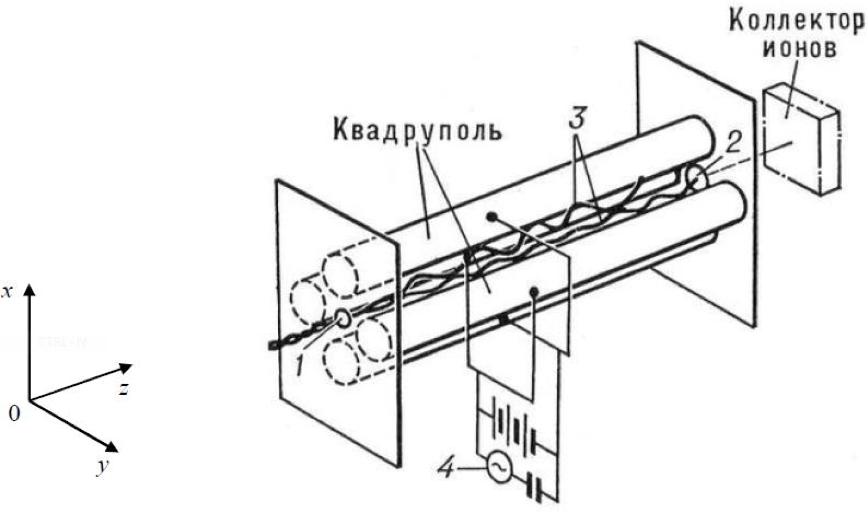
\includegraphics{quad.png}
		\caption{Схема квадрупольного масс-анализатора: 1 - входная апертура; 2 - выходная апертура; 3 - пучок ионов в анализаторе; 4 - генератор переменного напряжения.}
		\label{quad}
	\end{figure}\par
	Квадрупольный масс-анализатор относится к анализаторам с динамическим принципом действия. Он представляет собой квадрупольный конденсатор (рис. \ref{quad}), состоящий из четырех параллельных, симметрично расположенных проводящих стержней. К парам параллельных стержней приложены постоянное напряжение $U_0$ и переменное высокочастотное $U_\omega\cos\omega t$ ($\omega$ - частота, $t$ - время); их суммы для каждой пары равны по величине и противоположны по знаку.\par
	Действие такого анализатора состоит в том, что ионы, влетевшие в анализатор, движутся в камере анализатора вдоль оси $Oz$, параллельной продольным осям стержней, по сложным объемным спиралевидным траекториям, совершая поперечные колебания вдоль осей $x$ и $y$. При фиксированных значениях частоты и амплитуды переменного напряжения ионы с определенными значениями $m/Z$ проходят через квадрупольный конденсатор и попадают на коллектор; у ионов с другими значениями $m/Z$ амплитуда поперечных колебаний достигает такой величины, что они ударяются о стержни и разряжаются на них. Сканирование масс-спектра производится путем изменения постоянного и переменного напряжения (или частоты генератора). Для современных квадрупольных масс-спектрометров разрешающая способность достигает значения $R=10000$.
	\section{Практическая часть}
	\subsection{Ход работы}
	\begin{enumerate}
		\item Откачаем установку до высокого вакуума, включив последовательно форвакуумный и турбомолекулярный насосы. Убедимся по показанию вакуумметров, что вакуум не хуже, чем $10^{-4}$ Торр.
		\item Включаем компьютер. Управление установкой и квадпупольным масс-анализатором осуществляется с помощью специальных программ (SCADA и EasyView).
		\item Закроем клапан, отделяющий высоковакуумную часть установки от низковакуумной, теперь их соединяет только мембрана с отверстием 100 мкм. В низковакуумную часть установки будем напускать воздух из атмосферы ( 10, 20, 30 SCCM).
		\item Включим масс-спектрометр и получим спектр газов атмосферы в аналоговом виде  и в виде гистограммы. В работу помещены графики, изображенные в логарифмическом масштабе, т.к. они гораздо лучше отображают результаты эксперимента, чем графики в линейном масштабе.
		\item Выполнили дополнительное задание, в ходе которого пытались выяснить состав неизвестного вещества, которого напустили в систему.
	\end{enumerate}
	\subsection{Полученные результаты}
	\begin{enumerate}
		\item Таблица зависимости параметров $T_\text{атм}$, $T_\text{турбины}$, $I$, $N$ (обороты турбины), $P$ от времени:
		\begin{table}[h]
			\centering
			\begin{tabular}{|c|c|c|c|c|c|}
				\hline
				Время & $T_\text{атм}, ^\circ C$ & $T_\text{турбины},^\circ C$ & $I$, A & $N$ & $P$, Па\\
				\hline
				9:39 & 25 & 35 & 0.29 & 42046 & 8.9$\cdot 10^{-6}$\\
				9:44 & 25 & 37 & 0.28 & 42056 & 7.1$\cdot 10^{-6}$\\
				9:49 & 26 & 39 & 0.27 & 42056 & 5.4$\cdot 10^{-6}$\\
				9:54 & 27 & 40 & 0.27 & 42056 & 4.6$\cdot 10^{-6}$\\
				9:59 & 27 & 40 & 0.27 & 42060 & 4.0$\cdot 10^{-6}$\\
				10:04 & 27 & 41 & 0.26 & 42060 & 3.6$\cdot 10^{-6}$\\
				10:09 & 27 & 41 & 0.29 & 42056 & 2.2$\cdot 10^{-6}$\\
				\hline
			\end{tabular}
			\caption{Зависимость параметров установки от времени.}
		\end{table}
		\item Распределения для остаточных газов изображены на рис. \ref{bars}.
		\item Начнем напускать газ из баллона в установку и изучим изменения показаний. Распределения и графики после напускания изображены на рис. \ref{with_gas}.
		\begin{figure}[h]
			\centering
			\subfloat[Время: 9:39]{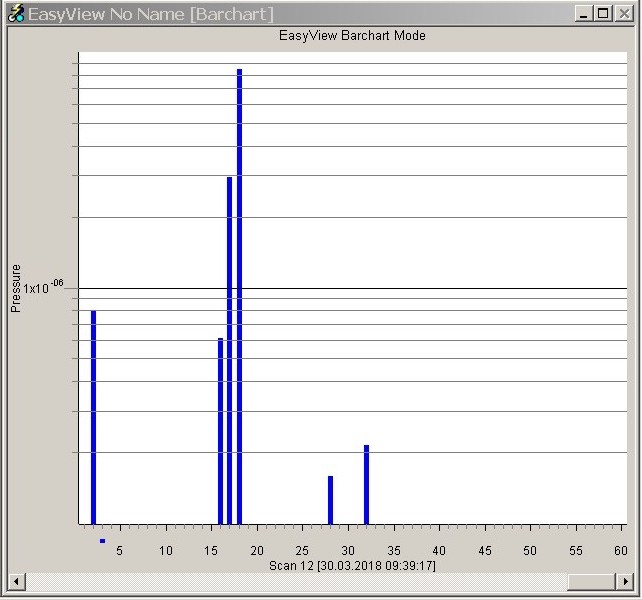
\includegraphics[scale=0.45]{2018-03-30_093938.jpg}}
			\qquad
			\subfloat[Время: 9:44]{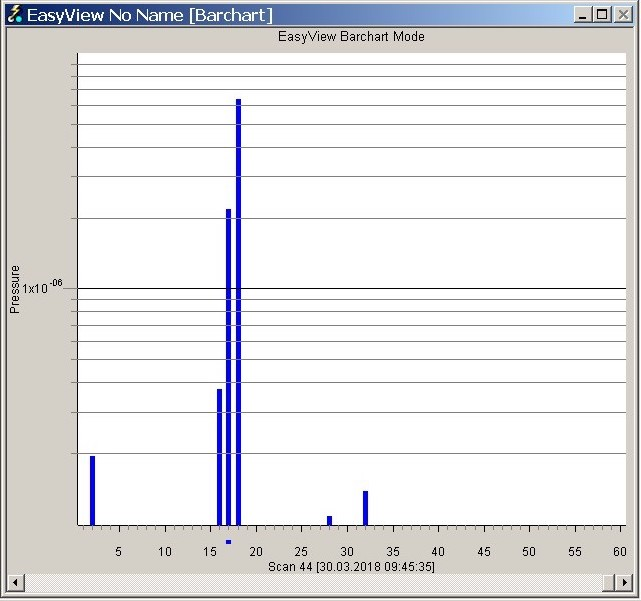
\includegraphics[scale=0.45]{2018-03-30_094556.jpg}}	
			
			\subfloat[Время: 9:49]{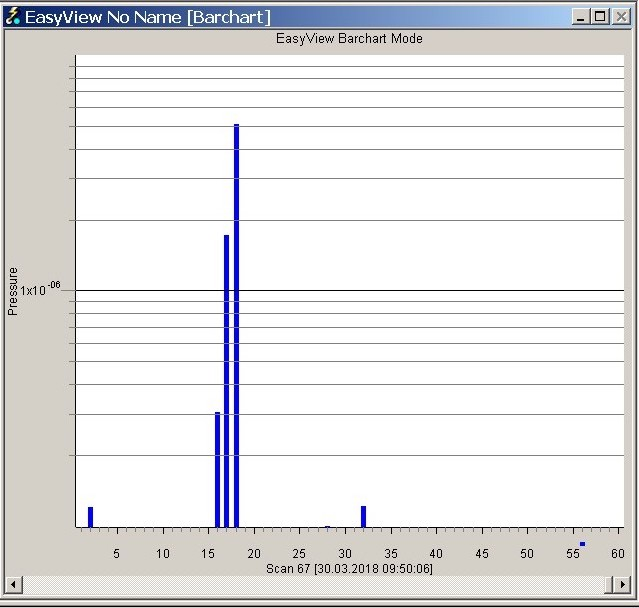
\includegraphics[scale=0.45]{2018-03-30_095032.jpg}}
			\qquad
			\subfloat[Время: 9:54]{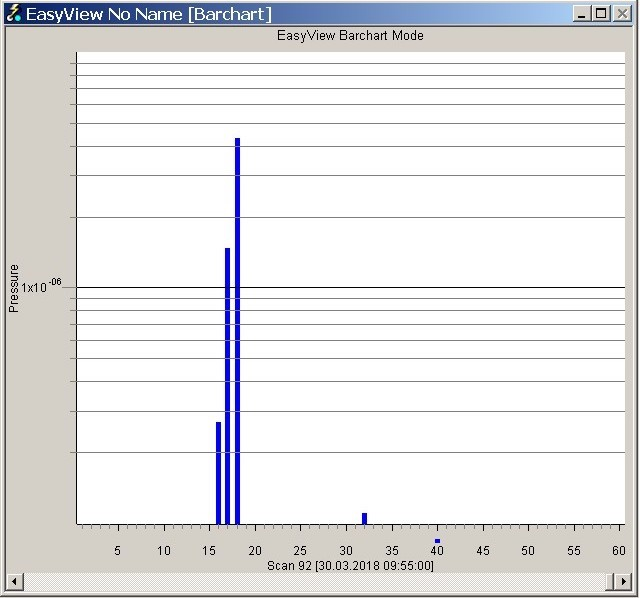
\includegraphics[scale=0.45]{2018-03-30_095524.jpg}}
			
			\subfloat[Время: 9:59]{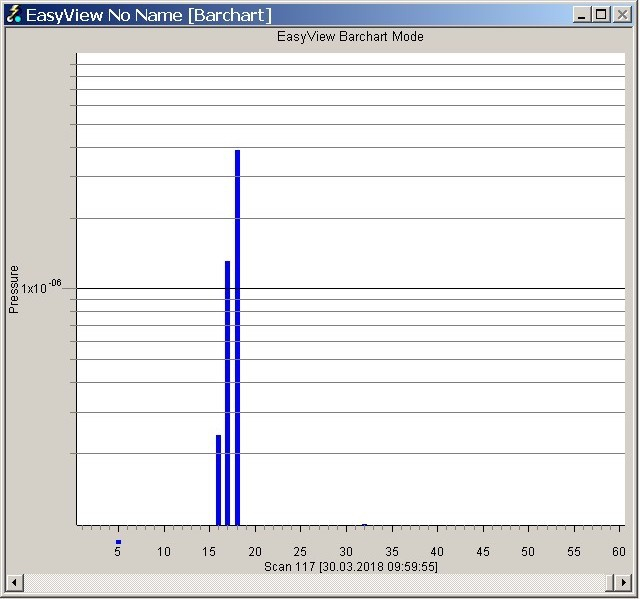
\includegraphics[scale=0.45]{2018-03-30_100017.jpg}}
			\qquad
			\subfloat[Время: 10:04]{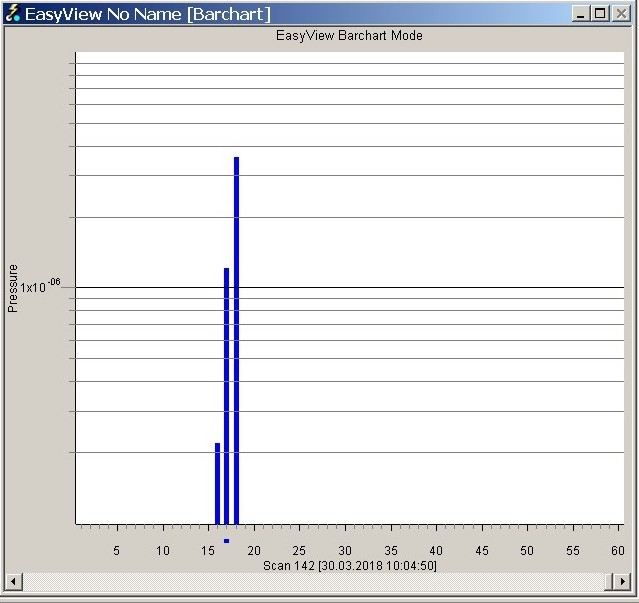
\includegraphics[scale=0.45]{2018-03-30_100510.jpg}}
			\caption{Распределения составляющих газов в различные моменты времени.}
			\label{bars}
		\end{figure}
		\begin{figure}
			\centering
			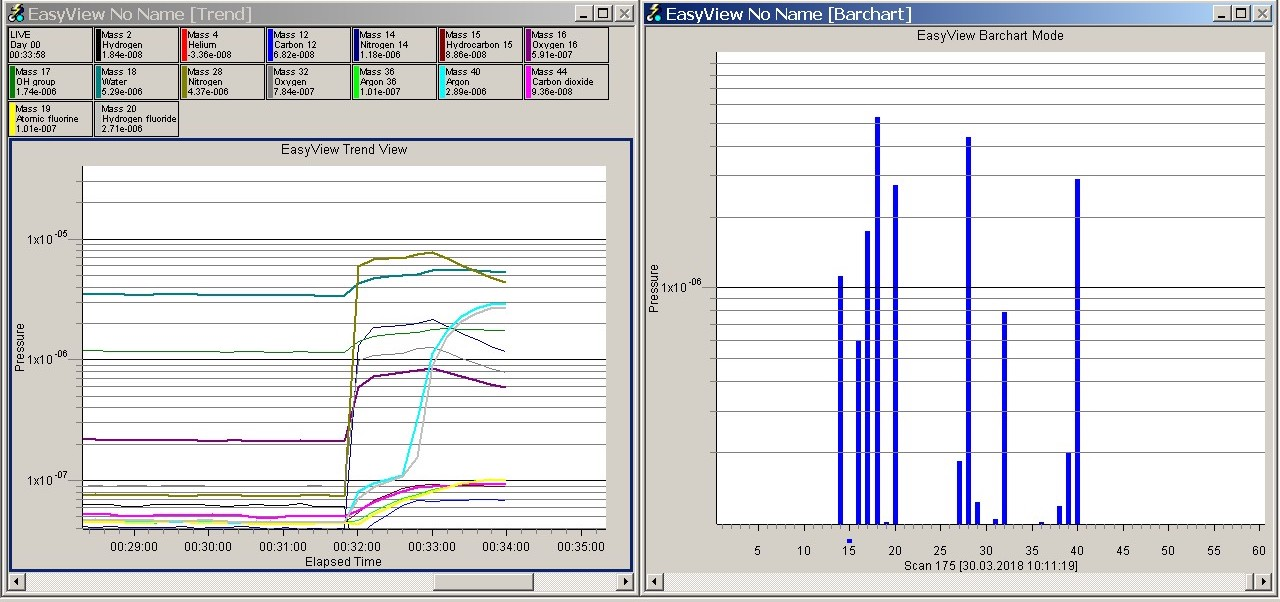
\includegraphics[scale=0.5]{2018-03-30_101140.jpg}
			\caption{Распределение после напускания газа из баллона.}
			\label{with_gas}
		\end{figure}
	\end{enumerate}
	\newpage
	\section{Выводы}
	\begin{enumerate}
		\item Ознакомились с работой квадрупольного масс-анализатора;
		\item Исследовали полученный масс-спектр остаточных газов в вакуумной установке;
		\item Напустили в вакуумный объем газ из баллона, получен масс-спектр газовой смеси;
		\item По расшифровке спектров можем говорить, что остаточный газ в вакуумной установке был схож по составу с воздухом(пики спектров приходятся на ионы воды),  исследуемый газ из баллона также схож по составу с воздухом(в связи с малым остатком заявленного газа в баллоне на начало работы.)
	\end{enumerate}
\end{document}
